\documentclass[fleqn]{article}
\usepackage[utf8]{inputenc}
\usepackage[letterpaper, total={7.5in, 10in}]{geometry}
\usepackage{amsmath}
\usepackage{amssymb}
\usepackage{relsize}
% \usepackage{tikz}
\usepackage[none]{hyphenat}
\usepackage{graphicx}
\usepackage{hyperref}
% \usetikzlibrary{matrix, positioning}

\title{\textbf{CSDS 435: Project 2}}
\author{John Mays, ``Group 13''}
\date{Due 04/04/23, Submitted 04/05/23; Dr. Li}

\begin{document}
\maketitle
\section{Introduction}
In this paper, I explore two (because I am one student) clustering methods along with two distance measures.  The two clustering methods I chose were k-Medoids and Complete-Link Hierarchical Clustering, because both accepted pre-generated distance kernels.  This went in line with the concurrent goal of also studying distance measures.  I compare the algorithms and the distance measures by metrics of separation and cohesion, and engage in hyperparameter tuning and visualization in order to explore these methods.
\section{Methods}
\subsection{Distance Measures}
\subsubsection{Normalized Unordered Edit Distance}
$$d_{1}(x,y)=\frac{\sum_{k}x_k-y_k}{\sum_{k}x_k+y_k}$$
The intuition behind this was, when I was considering how you compare strings, I was reminded of edit distance (both for words and sentences).  Of course, I realized that edit distance required an ordered string, and our bag-of-words model doesn't preserve the order.  But I thought, very simply, the difference between two vectors is essentially a version of edit distance that does not pay attention to order (hence ``unordered'').  But I also thought two four-word sentences with two words in common are about as near as two six-word sentences with three words in common, or at least that this might be a good hypothesis to test since my other distance measure \textit{does not} treat the data this way.  Hence, I normalize the distance by dividing by the total number of words in both.  This distance measure is $\frac{\text{\# of words not in common}}{\text{\# total number of words in both sentences}}$.  Therefore, the minimum value ($d_{1}(x,x)$) is zero, and the maximum value (for vectors with no words in common) is one.

\subsubsection{Euclidean Distance}
$$d_{2}(x,y)=\sqrt{\sum_{k}(x_k-y_k)^{2}}$$
Euclidean distance seemed intuitive.  It will, as opposed to my first distance measure, attribute greater distances on average to longer tweets.  Two sixty-word tweets will be much farther apart than two ten-word tweets (assuming they each have nothing in common).
\subsubsection{Comparisons}
The distributions are extremely different.  The Euclidean distance's ($d_{2}$) is almost normal with $\mu \approx 4$, while $d_{1}$ has an extraordinary amount of 1.0 (no words in common) and then just a few thousand distances clustered around 0.9.
\begin{center}
	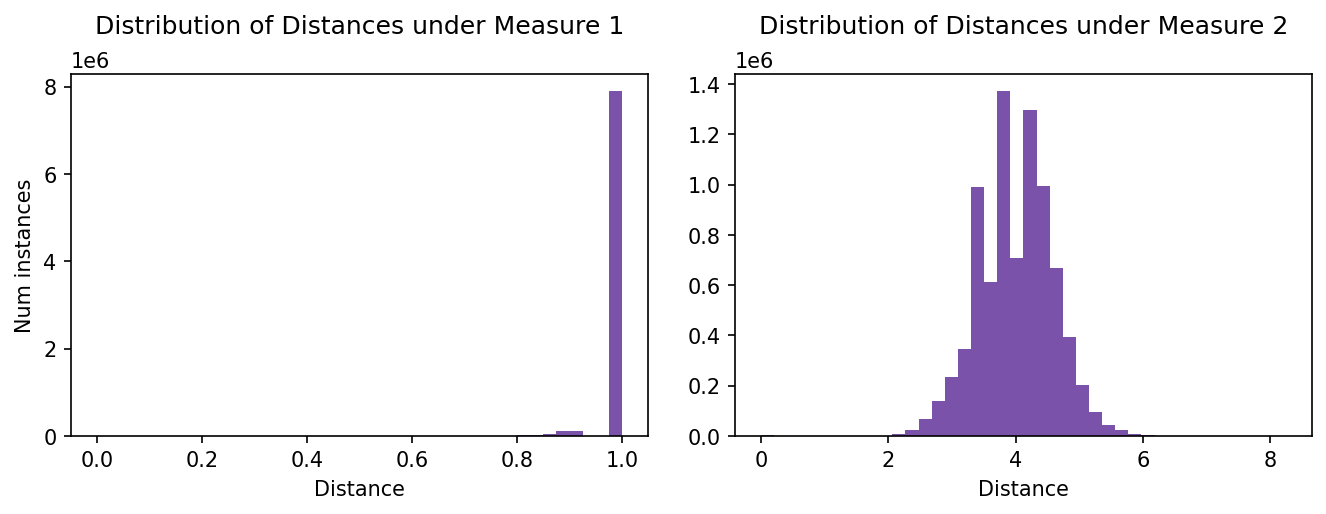
\includegraphics[scale=0.50]{images/distance_distributions_horizontal.png}
\end{center}

\subsection{Choosing Hyperparameters}
\subsubsection{Choosing $k$ for k-Medoids:}
\begin{center}
	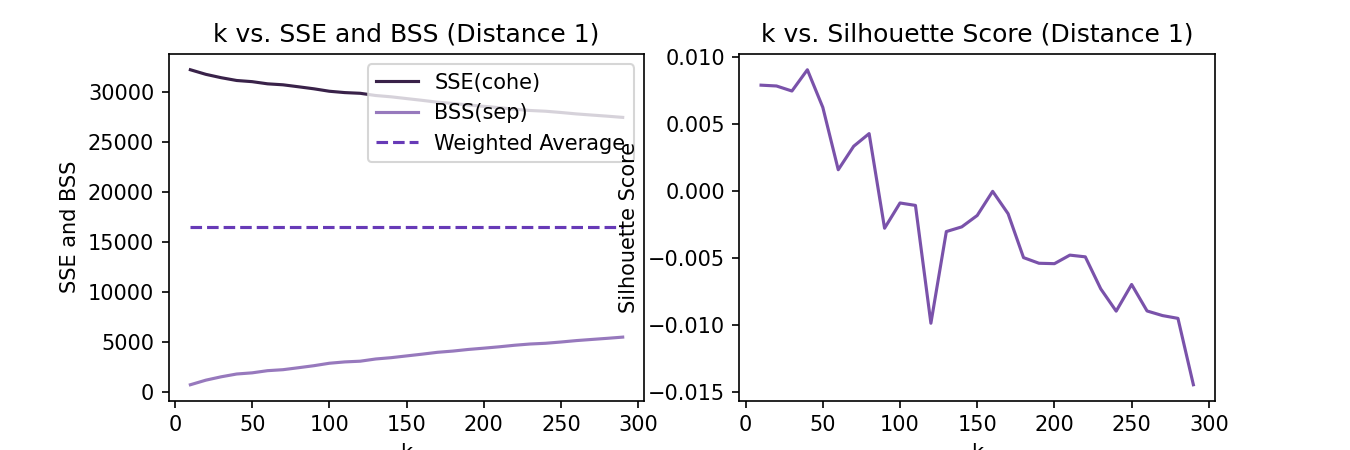
\includegraphics[scale=0.40]{images/d1_ks.png}
	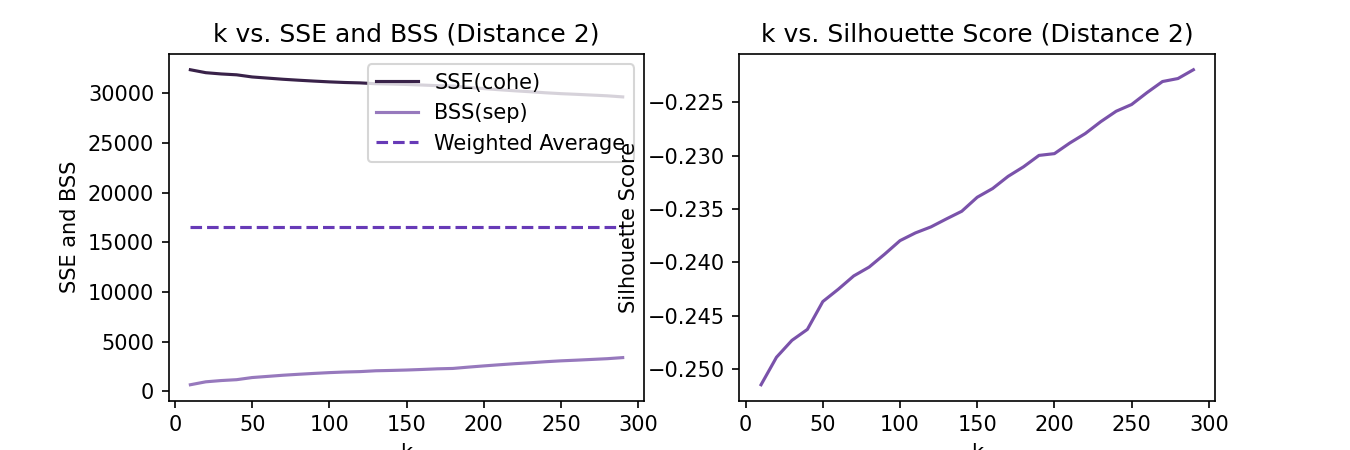
\includegraphics[scale=0.40]{images/d2_ks.png}
\end{center}

\subsubsection{Choosing $k$ for Hierarchical:}
\begin{center}
	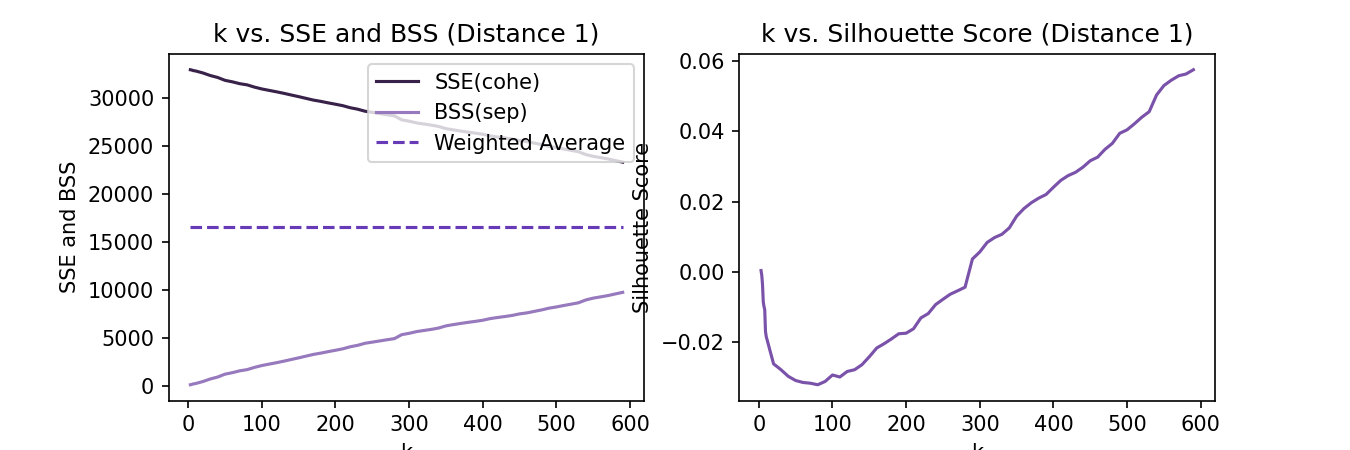
\includegraphics[scale=0.40]{images/d1_f_ks.png}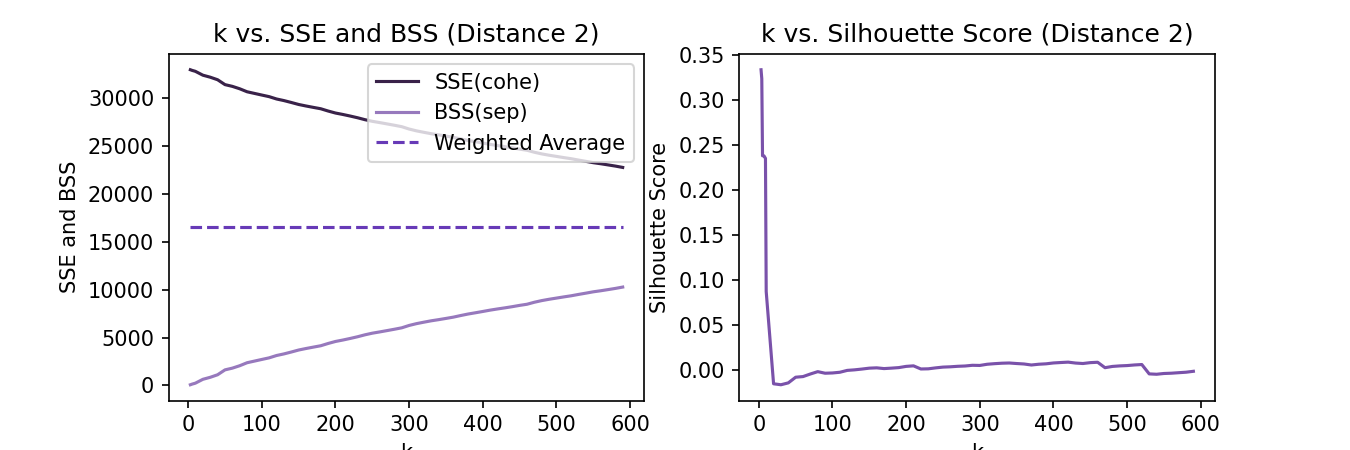
\includegraphics[scale=0.40]{images/d2_f_ks.png}
\end{center}
Both of my methods required me to choose $k$ (number of clusters).  In order to do this, I tried to observe how different metrics and objective functions varied with $k$.  Some results were surprising, and revealed to me that different distances worked very differently with different clustering algorithms.  Observing $SSE$ and $BSS$ turned out not to be very helpful, but observing the silhouette score was.  In general, a silhouette score closer to one is better.  The only two combinations that demonstrated a positive correlation between silhouette score and k were \{Distance 1 and Hierarchical\} and \{Distance 2 and k-Medoids\}. The other two were negatively correlated, and less so.  For $k$-Medoids I chose a default $k$ of 50 as that is the max silhouette achieved with either distance.  And for Hierarchical, smaller choices were not giving me coherent clusters, so I chose a much higher $k$ based on the $d_1$ figure: 600.
\section{Data}
\subsection{Dataset Summary}
\begin{tabular}{|c|c|c|c|}
	\hline
	\textbf{\# Num of Tweets} & \textbf{\# Num of Words (total)} & \textbf{\# Num of Tokens} & \textbf{\# Avg Num of Words}\\
	\hline
	4,061&32,612&9,609&8.031\\
	\hline
\end{tabular}
\subsubsection*{Top Ten Legal Tokens:}
``health'', ``getfit'', ``new'', ``$@$cnnhealth'', ``today's'', ``cancer'', ``know'', ``kids'', ``$@$drsanjaygupta'', ``ebola''
%\begin{minipage}{0.5\textwidth}
%	\begin{enumerate}
%%    	\item \textit{``health''}
%    	\item \textit{``getfit''}
%    	\item \textit{``new''}
%   	\item \textit{``@cnnhealth''}
%    	\item \textit{``today's''}
%	\end{enumerate}
%\end{minipage}
%\begin{minipage}{0.5\textwidth}
%	\begin{enumerate}
%   	\item[6.] \textit{``cancer''}
%    	\item[7.] \textit{``know''}
%    	\item[8.] \textit{``kids''}
%    	\item[9.] \textit{``@drsanjaygupta''}
%    	\item[10.] \textit{``ebola''}
%	\end{enumerate}
%\end{minipage}


\subsection{Stopwords:}
% old # of words: 48,233
Initially, I tried manual stopword selection, but I found this task to be cumbersome, and to leave in less frequent stopwords that were still important.  So I chose most of the stopwords from the \textit{Natural Language Toolkit }(NLTK), electing to leave a certain few out, while also trying my best to include ones specific to the dataset.  After subtracting the NLTK words, I scanned through the most popular 100 words still left.  The words \textit{``rt''} (retweet) and \textit{``w/''} (with) were removed, along with spurious characters that somehow made it through my regex cleaning.\\
\newline
When choosing what to keep and what to toss, I had a hard time deciding.  Common stopwords like \textit{``was''} and \textit{``is''} contain tense information that could hypothetically be related to a cluster's meaning, but I chose to go with precedent, which suggests that they are more noise than they are worth.  I elected to remove the URLs since they were almost never in common between tweets.  However, I chose to leave ``@'' mentions and ``hashtags'' in.  I removed the hashtag character, however, as I judged ``\#ebola'' and ``ebola'' could be treated as one in the same. Hashtags and \textit{``@''}-mentions were left in because I thought that clusters could potentially be formed around them.  Quite often, a hashtag's sole purpose is to distill the subject or message of the tweet.  And although not all textit{``@''}-mentions feature a certain doctor or expert, the ones that do and are the same are intrinsically related to one another.

\section{Results}
\textbf{k-Medoids with }$\mathbf{d_1}$:\\
\begin{minipage}{0.65\textwidth}
	\begin{tabular}{|c|c|c|c|}
    	\hline
    	\textbf{Number of Clusters} & \textbf{SSE} &\textbf{BSS} &\textbf{Silhouette Score}\\
    	\hline
    	50 & 31061.623 & 1960.594 & 0.006\\
    	\hline
	\end{tabular}
\end{minipage}\begin{minipage}{0.35\textwidth}
	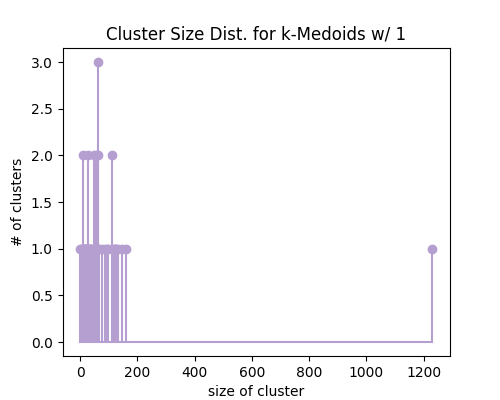
\includegraphics[scale=0.35]{images/size_dist_km_d1.png}
\end{minipage}\\
\textbf{k-Medoids with }$\mathbf{d_2}$:\\
\begin{minipage}{0.65\textwidth}
	\begin{tabular}{|c|c|c|c|}
    	\hline
    	\textbf{Number of Clusters} & \textbf{SSE} &\textbf{BSS} &\textbf{Silhouette Score}\\
    	\hline
    	50 & 31631.14 & 1391.078 & -0.244\\
    	\hline
	\end{tabular}
\end{minipage}\begin{minipage}{0.35\textwidth}
	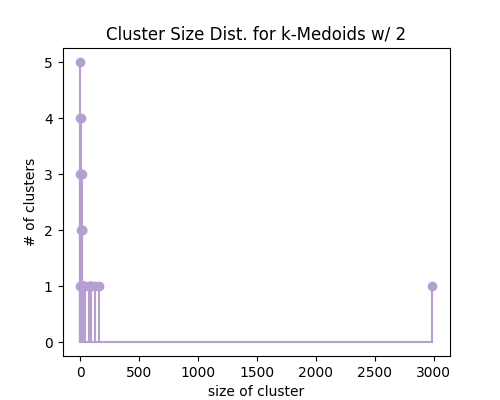
\includegraphics[scale=0.35]{images/size_dist_km_d2.png}
\end{minipage}\\
\textbf{Hierarchical with }$\mathbf{d_1}$:\\
\begin{minipage}{0.65\textwidth}
\begin{tabular}{|c|c|c|c|}
	\hline
	\textbf{Number of Clusters} & \textbf{SSE} &\textbf{BSS} &\textbf{Silhouette Score}\\
	\hline
	600 & 23151.933 & 9870.284 & 0.058\\
	\hline
\end{tabular}
\end{minipage}
\begin{minipage}{0.35\textwidth}
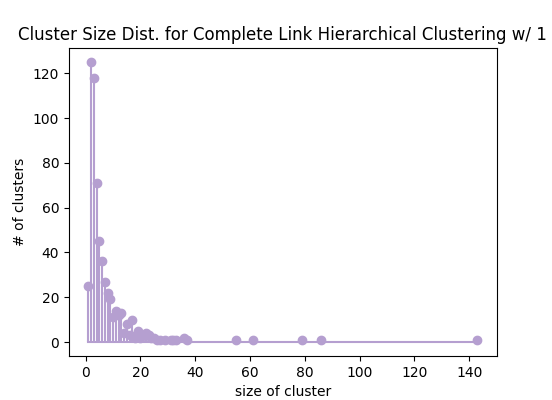
\includegraphics[scale=0.35]{images/size_dist_hc_d1.png}\end{minipage}\\
\textbf{Hierarchical with }$\mathbf{d_2}$:\\
\begin{minipage}{0.65\textwidth}
\begin{tabular}{|c|c|c|c|}
	\hline
	\textbf{Number of Clusters} & \textbf{SSE} &\textbf{BSS} &\textbf{Silhouette Score}\\
	\hline
	600 & 22643.094 & 10379.124 & -0.001\\
	\hline
\end{tabular}
\end{minipage}
\begin{minipage}{0.35\textwidth}
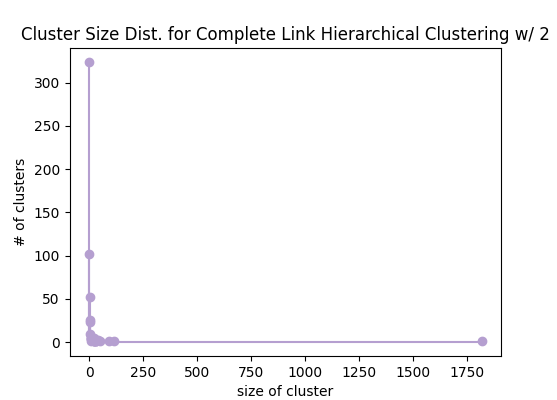
\includegraphics[scale=0.35]{images/size_dist_hc_d2.png}\end{minipage}\\
\subsection*{Cluster Deciphering}
For Complete-Link Hierarchical Clustering, I had what looked like the best clusters, so here some of them are:\\
\underline{Note:} this was run with $k=600$ and $d_1$.\\
\newline
\begin{tabular}{|c|c|c|c|c|}
	\hline
	\textbf{Cluster:} &\textbf{Cluster 3}& \textbf{Cluster 1}&\textbf{Cluster 109}&\textbf{Cluster 86}\\
	\hline
	\textbf{size:}& 143 & 86 & 61&55\\
	\hline
	\textbf{Popular tokens:}& getfit& health&cancer&ebola\\
	&today's&minute&breast&american\\
	&eat&insurance&one&$@$jechristensen\\
	&make&good&survival&infected\\
	&eating&weight&scary&$@$elizcohencnn\\
	&calories&crisis&prevent &ebolaqanda\\
	&$@$shape\_magazine&today's&new& $@$who\\
	&day&loss&come &patients\\
	&every&know&@cnnhealth &like \\
	&healthy&food&you?&experimental\\
	\hline
\end{tabular}\\
\newline
There are some really nice clusters here. \textbf{Cluster 3} has a prevailing theme of diet and weight loss.  \textbf{Cluster 1} seems to be about modern weight problems. \textbf{Cluster 109} is mostly scare-tweets about breast cancer and survival rates.  \textbf{Cluster 86} is about the ebola outbreak in America.
\subsection{Cluster Visualizations:}
Since there are several thousand pixels, and the details are finer, the sorted distance matrices can be found in the appendix at a large scale\dots
\subsection{Cluster Consistency:}
I used entropy and purity to compare k-Medoids to Complete Link Hierarchical Clustering, both using distance measure 2 (Euclidean).  Here are my results:
\begin{itemize}
	\item When k-Medoids is the label, Entropy = 0.822, Purity = 0.81
	\item When Complete Link Hierarchical Clustering is the label, Entropy = 3.164, Purity = 0.457
\end{itemize}

\section{Conclusion}
Even with our self-imposed limitation of only kernel methods, we managed to run a successful comparison and try a somewhat novel distance measure.  Keeping the limited scope of this report in mind, at least on my two distance measures, Hierarchical clustering (with Complete Linkage) seemed to consistently outperform k-Medoids in measures of cohesion and separation, silhouette score, and common understanding.  The clustering was generally much more coherent coming from Hierarchical Clustering, \textit{especially} with distance metric one.  Although this report is by no means a complete dive into clustering, let alone these two metrics, it gave us some insight into how the two methods work in limited cases, and despite having an upsetting-looking distribution at first, novel distance measure $d_1=$ Normalized Unordered Edit Distance proved functional and excelled against Euclidean distance.


\section*{Statement of Participation}
\begin{itemize}
	\item John Mays: $100\%$
\end{itemize}
All team members agree with the specified effort.

\section*{Sources}
$[1]$ \href{https://towardsdatascience.com/text-pre-processing-stop-words-removal-using-different-libraries-f20bac19929a}{\textit{Text pre-processing: Stop words removal using different libraries(NLTK)}}\\
$[2]$ \textit{Introduction to Data Mining (2nd ed.)} Tan et al.\\
$[3]$ \href{https://arxiv.org/abs/1705.00995}{\textit{Fuzzy Approach Topic Discovery in Health and Medical Corpora} by Karami, Gangopadhyay, Zhou, and Kharrazi}
\pagebreak
\section*{Appendix}
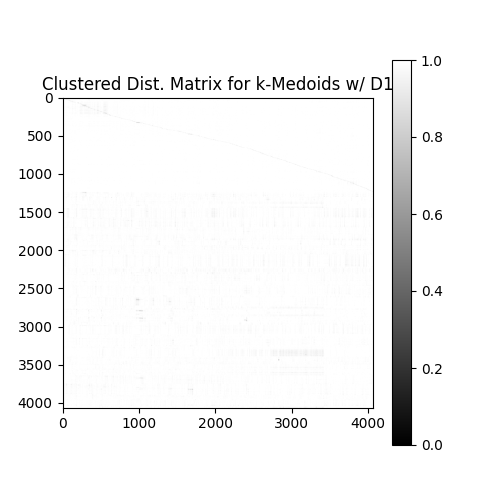
\includegraphics[scale=1]{images/dist_matrix_km_d1.png}\\
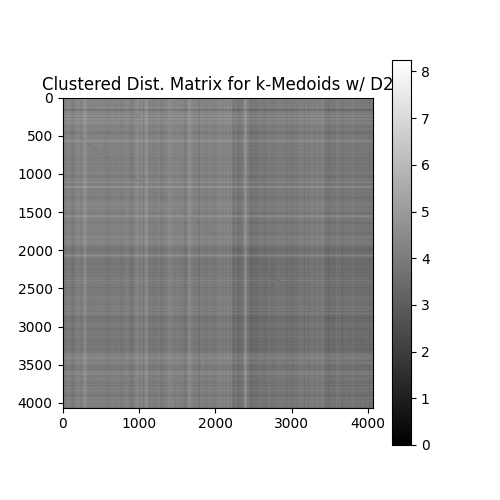
\includegraphics[scale=1]{images/dist_matrix_km_d2.png}\\
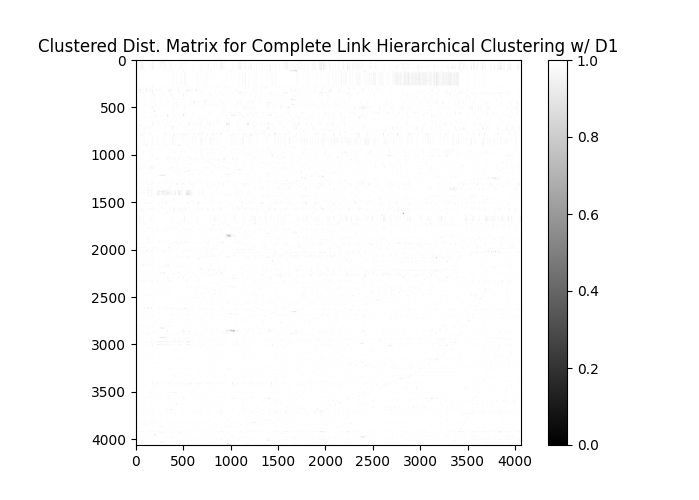
\includegraphics[scale=0.8]{images/dist_matrix_hc_d1.png}\\
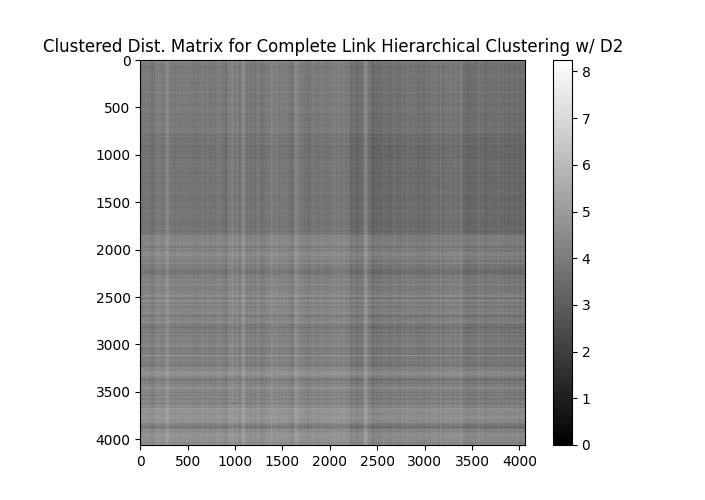
\includegraphics[scale=0.8]{images/dist_matrix_hc_d2.png}\\
\end{document}